%%%%%%%%%%%%%%%%%%%%%%%%%%%%%%%%%%%%%%%%%%%%%%%
%%%%%%%%%%%%%%%%%%%%%%%%%%%%%%%
\documentclass{l3deliverable}
%%%%%%%%%%%%%%%%%%%%%%%%%%%%%%%%%%%%%%%%%%%%%%%
%%%%%%%%%%%%%%%%%%%%%%%%%%%%%%%
\usepackage{graphicx}%
\usepackage{tabularx}%
\usepackage{url}%
\usepackage{usecasedescription}%
%%%%%%%%%%%%%%%%%%%%%%%%%%%%%%%%%%%%%%%%%%%%%%%
%%%%%%%%%%%%%%%%%%%%%%%%%%%%%%%
%% Check these macro values for appropriateness for your own document.
\title{Requirements Document}
\author{Ross Adam\\
Andrew Gardner\\
Nicole Kearns\\
Mamas Nicolaou\\
Asset Sarsengaliyev\\
}
\date{1st November 2012}
\deliverableID{D3}
\project{PSD3 Group Exercise 1}
\team{V}
\version{1.0}
%%%%%%%%%%%%%%%%%%%%%%%%%%%%%%%%%%%%%%%%%%%%%%%
%%%%%%%%%%%%%%%%%%%%%%%%%%%%%%%
\begin{document}
%%%%%%%%%%%%%%%%%%%%%%%%%%%%%%%%%%%%%%%%%%%%%%%
%%%%%%%%%%%%%%%%%%%%%%%%%%%%%%%
\maketitle
\tableofcontents
\newpage
%%%%%%%%%%%%%%%%%%%%%%%%%%%%%%%%%%%%%%%%%%%%%%%
%%%%%%%%%%%%%%%%%%%%%%%%%%%%%%%
%% Standard section for all documents
\section{Introduction}

\subsection{Identification}

Requirements specification for the internship system for PSD3 team project.
\subsection{Related Documentation}

PSD3 Group Exercise Description \url{http://fims.moodle.gla.ac.uk/file.php/128/coursework/
psd3-ge-1-rev3278.pdf}\\
Deliverables Template \url{http://fims.moodle.gla.ac.uk/file.php/128/coursework/templates.zip}\\
PSD3 Course Notes \url{http://fims.moodle.gla.ac.uk/file.php/128/lecture-notes/notes-r3275.pdf}
\\
\subsection{Purpose and Description of Document}

The purpose of this document is to detail and explain the requirements collected for the
internship advert system. This will include all the actors within the system, their use cases and
descriptions, and scenarios which would be suitable for the system.
%%%%%%%%%%%%%%%%%%%%%%%%%%%%%%%%%%%%%%%%%%%%%%%
%%%%%%%%%%%%%%%%%%%%%%%%%%%%%%%

\subsection{Document Status and Schedule}

\begin{center}{
\begin{tabular}{|c|c|c|c|}
\hline \textbf{Date} &\textbf{ Change} & \textbf{Version} & \textbf{Author}\\ 
\hline 25/10/2012 & Began Draft & 0.1 & All \\ 
\hline 30/10/2012 & Initial Draft Completed & 0.2 & All \\ 
\hline 10/11/2012 & Finalised for Submission & 0.3 & All\\ 
\hline 11/11/2012 & \textbf{Draft Submission Deadline} & 1.0 & All\\ 
\hline ... & Revision & & All\\ 
\hline 19/11/2012 & Modified Section 4 & 1.1 & Nicole\\
\hline 26/11/2012 & Modified the use case diagrams & 1.2 & Nicole\\
\hline 26/11/2012 & Modified the use case descriptions & 1.3 & Andrew\\
\hline 27/11/2012 & Modified the use case scenarios & 1.4 & Nicole\\
\hline 27/11/2012 & & &\\
\hline 29/11/2012 & \textbf{Final Submission Deadline} & & All\\ 
\hline 
\end{tabular} }
\end{center}

\section{Extended Problem Definition}
A program is needed to manage internship adverts posted by companies that students can then
search through and then apply if they are interested.
In order for this program to be successful it requires a login system that allows a company
to submit, edit or remove their adverts. Submitted adverts are then reviewed by the Course
Co-ordinator. If deemed relevant they will be added to the list of adverts for students to see.
Applying will send the student’s details to the company to register their interest. The course co-
ordinator will remove any adverts that have been filled or whose deadlines have expired.\\
%%%%%%%%%%%%%%%%%%%%%%%%%%%%%%%%%%%%%%%%%%%%%%%
%%%%%%%%%%%%%%%%%%%%%%%%%%%%%%%
\section{System Scope}

%%%%%%%%%%%%%%%%%%%%%%%%%%%%%%%%%%%%%%%%%%%%%%%
%%%%%%%%%%%%%%%%%%%%%%%%%%%%%%%

\subsection{System Actors}
\textbf{Course Coordinator}: Responsible for the management of adverts on the system.\\
\textbf{Students}: Uses the system to browse the list of internship adverts and apply.\\
\textbf{Company}: Submits adverts for moderation.\\

%%%%%%%%%%%%%%%%%%%%%%%%%%%%%%%%%%%%%%%%%%%%%%%
%%%%%%%%%%%%%%%%%%%%%%%%%%%%%%%

\subsection{Domain Model}

%\begin{figure}[h]
%\begin{center}
%\includegraphics
%[scale=0.7]
%{/users/level3/0902059k/Level3/PSD3/Deliverables/Images/UML.png}
%\caption{Domain model}
%\label{fig1:domain model}
%\end{center}
%\end{figure}

%%%%%%%%%%%%%%%%%%%%%%%%%%%%%%%%%%%%%%%%%%%%%%%
%%%%%%%%%%%%%%%%%%%%%%%%%%%%%%%

\section{Use Case Descriptions}

This section describes the required functionality for the Student Internship Advert System as
four groups of related
use cases. The core use cases for the system are:\\

\textbf{Submission of internship advertisements (Section 4.1):}
\begin{itemize}
\item Submit internship adverts
\item Edit adverts 
\end{itemize}

\textbf{Review, comment and publication of internship advertisements by Course Coordinator
(Section 4.2) :}
\begin{itemize}
\item Review internship adverts
\item Approve internship adverts
\end{itemize}

\textbf{Review of Advertisement by Student (Section 4.3) :}
\begin{itemize}
\item Review internship adverts list
\item Apply for internship
\end{itemize}

\textbf{Notification of successful selection for an internship by an SE/ESE student (Section 4.4)
:}
\begin{itemize}
\item Notify course coordinator of successful placement
\item remove internship adverts
\end{itemize}

\textbf{Common utility services (Section 4.5) :}
\begin{itemize}
\item Login
\item Logout
\end{itemize}

\subsection{Submission of internship advertisements}
\begin{figure}[h]
\begin{center}
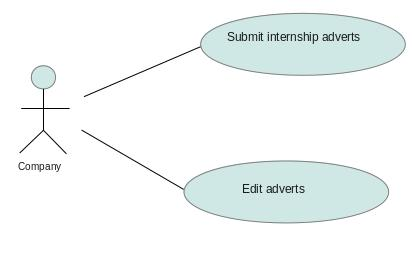
\includegraphics
[scale=0.7]
{Company.jpeg}
\caption{Use Case Diagram 4.1}
\label{fig2:Use Case Diagram4.1}
\end{center}
\end{figure}

\begin{UseCaseTemplate}
\UseCaseLabel{Submit internship adverts}
\UseCaseDescription{A company should login and post internship adverts to the system,
confirm it and logout.}
\UseCaseRationale{A company must be able to submit internship adverts to the system in order for the students to view and apply for the placement.}
\UseCasePriority{Must have}
\UseCaseStatus{Not implemented}
\UseCaseActors{Company}
\UseCaseIncludes{Login,Logout}
\UseCaseConditions{Post: The advert is then stored and must be approved by the CC before put on the system for students to view.}
\UseCaseNonFunctionalRequirements{}
\UseCaseScenarios{A company logs in to the system and fills out the advert form, filling in all appropriate details, and then submits it for review by the course coordinator.}
\UseCaseRisks{}
\end{UseCaseTemplate}

\begin{UseCaseTemplate}
\UseCaseLabel{Edit adverts}
\UseCaseDescription{A company must login, make changes to their advert where necessary,
confirm changes and then logout.}
\UseCaseRationale{A company must be able to make changes to their advert in order to include
more information about it or remove irrelevant/incorrect details.}
\UseCasePriority{Must Have}
\UseCaseStatus{Not implemented}
\UseCaseActors{Company}
\UseCaseIncludes{Login,Logout}
\UseCaseConditions{Pre: Company must have uploaded their advert to the system. Post: The
amended advert will now be reviewed (again) by the course Coordinator.}
\UseCaseNonFunctionalRequirements{}
\UseCaseScenarios{The company logs in. They select the option to edit their advert, and selcts which section they want to edit. The appropriate changes are made and the advert must wait for approval by the CC.}
\UseCaseRisks{}
\end{UseCaseTemplate}

\subsection{Review, comment and publication of internship advertisements by Course
Coordinator}

\begin{figure}[h]
\begin{center}
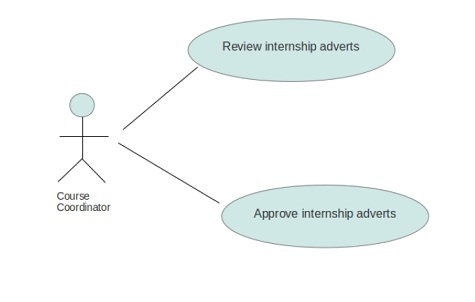
\includegraphics
[scale=0.7]
{CourseCoordinator.jpg}
\caption{Use Case Diagram 4.2}
\label{fig2:Use Case Diagram4.2}
\end{center}
\end{figure}

\begin{UseCaseTemplate}
\UseCaseLabel{Review internship adverts}
\UseCaseDescription{Course coordinator must login, read through new/edited adverts posted
and decide if they are suitable for the students.}
\UseCaseRationale{A member of the school of computing science (course coordinator) must
review all adverts to ensure they are suitable for ESE/SE students.}
\UseCasePriority{Must have}
\UseCaseStatus{Not implemented}
\UseCaseActors{Course Coordinator}
\UseCaseIncludes{Login,Logout}
\UseCaseConditions{ Pre: company must post adverts to the system. Post: adverts are made
available to the students.}
\UseCaseNonFunctionalRequirements{}
\UseCaseScenarios{The CC logs into the system. The CC will view all unapproved adverts submitted to the system and decide whether or not the internship is suitable for the students. If not, the advert is not made available to the students and is removed from the system.}
\UseCaseRisks{}
\end{UseCaseTemplate}
\begin{UseCaseTemplate}

\UseCaseLabel{Approve internship adverts}
\UseCaseDescription{Course Coordinator must login. After reviewing the adverts and deciding
they are suitable, the adverts are made available to the students.}
\UseCaseRationale{A member of the school of computing science (course coordinator) is
responsible for making adverts available for the students so they can view and apply for the
internships.}
\UseCasePriority{Must have}
\UseCaseStatus{Not implemented}
\UseCaseActors{Course coordinator}
\UseCaseIncludes{Login,Logout}
\UseCaseConditions{ Pre: company upload adverts to the system. Pre: adverts reviewed by
course coordinator}
\UseCaseNonFunctionalRequirements{}
\UseCaseScenarios{The CC logs in to the system. The CC will then select the option to view unapproved adverts. After reviewing the advert, the  CC selects yes and states which students this advert is suitable for.}
\UseCaseRisks{Course coordinator may accidentally approve an unsuitable advert.}
\end{UseCaseTemplate}

\subsection{Review of Advertisement by Student}

\begin{figure}[h]
\begin{center}
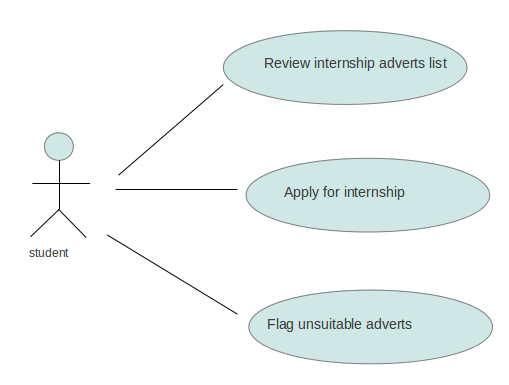
\includegraphics
[scale=0.7]
{Student.jpeg}
\caption{Use Case Diagram 4.3}
\label{fig2:Use Case Diagram4.3}
\end{center}
\end{figure}

\begin{UseCaseTemplate}
\UseCaseLabel{Review internship adverts list}
\UseCaseDescription{List of adverts is displayed on screen and users scrolls through and can
read detailed information about the internship.}
\UseCaseRationale{User needs to be able to see the adverts in order to apply.}
\UseCasePriority{Must Have}
\UseCaseStatus{Not Implemented}
\UseCaseActors{Student}
\UseCaseIncludes{Login, Logout, Apply for internship}
\UseCaseConditions{Pre: adverts have been approved by the CC.}
\UseCaseNonFunctionalRequirements{}
\UseCaseScenarios{}
\UseCaseRisks{}
\end{UseCaseTemplate}

\begin{UseCaseTemplate}
\UseCaseLabel{Apply for internship}
\UseCaseDescription{User selects an advert to apply for and will then have to email the
company or will be directed to the company website to apply}
\UseCaseRationale{Student should be redirected to the company URL or email in order to apply for the internship placement.}
\UseCasePriority{Must Have}
\UseCaseStatus{Not Implemented}
\UseCaseActors{Student}
\UseCaseIncludes{Login,Logout}
\UseCaseConditions{}
\UseCaseNonFunctionalRequirements{}
\UseCaseScenarios{The student will select the apply option within the system. The student will then be redirected to the company website in order to fill out the application for the internship.}
\UseCaseRisks{The email/website may be incorrect so student may not be able to apply.}
\end{UseCaseTemplate}

\subsection{Notification of successful selection for an internship by an SE/ESE student}

\begin{figure}[h]
\begin{center}
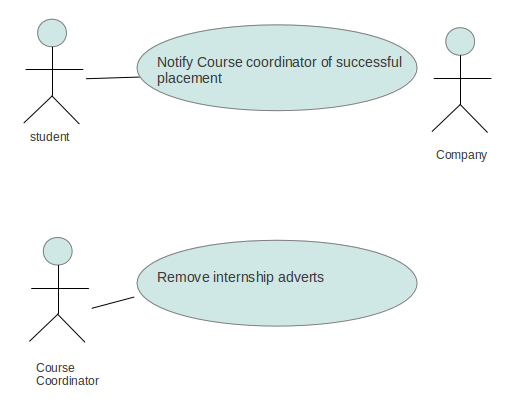
\includegraphics
[scale=0.7]
{Section4.jpeg}
\caption{Use Case Diagram 4.4}
\label{fig2:Use Case Diagram4.4}
\end{center}
\end{figure}

\begin{UseCaseTemplate}
\UseCaseLabel{Notify course coordinator of successful placement}
\UseCaseDescription{Let course coordinator know a Placement position has been filled.}
\UseCaseRationale{A student should let the Course Coordinator know that they were successful
with their application for a specified placement position so that the CC can go on and remove
the advert from the System.}
\UseCasePriority{Must have.}
\UseCaseStatus{Not Implemented}
\UseCaseActors{Student}
\UseCaseIncludes{Login,Logout}
\UseCaseConditions{Pre: The advert for the placement position that was taken must be still
visible on the system. Post: Course Coordinator is notified.}
\UseCaseNonFunctionalRequirements{}
\UseCaseScenarios{A student has been successful with a placement with one of the adverts on the system. The student will notfiy the Course coordinator of there successful placement within the system and the course coordinator will receive an email.}
\UseCaseRisks{}
\end{UseCaseTemplate}

\begin{UseCaseTemplate}
\UseCaseLabel{remove internship adverts}
\UseCaseDescription{Course Coordinator logins in to system. If advert is passed deadline or no
longer suitable or available, the advert will be taken off the system and then log out.}
\UseCaseRationale{A member of the school of computing science (course coordinator) is
responsible for taking adverts down so as to avoid students applying for internships that are no
longer available or suitable.}
\UseCasePriority{Must have}
\UseCaseStatus{Not implemented}
\UseCaseActors{Course coordinator}
\UseCaseIncludes{Login,Logout}
\UseCaseConditions{Pre: Course Coordinator has recieved a notification to say the placement has been filled. Post: Advert no longer available on the system.}
\UseCaseNonFunctionalRequirements{}
\UseCaseScenarios{The course coordinator has recieved a notification of a successful placement and logs into the system. The course coordinator then removes the internship advert from the system, so that it is no longer available to the students.}
\UseCaseRisks{Course Coordinator might remove the wrong advert.}
\end{UseCaseTemplate}

\subsection{Common utility services}

\begin{UseCaseTemplate}
\UseCaseLabel{Login}
\UseCaseDescription{A user should enter their login id and a password to allow them to access
the system. }
\UseCaseRationale{A user must be able to login, providing different levels of access to the system.}
\UseCasePriority{Must have}
\UseCaseStatus{Not implemented}
\UseCaseActors{Company, Students, Course Coordinator}
\UseCaseIncludes{}
\UseCaseConditions{}
\UseCaseNonFunctionalRequirements{}
\UseCaseScenarios{}
\UseCaseRisks{}
\end{UseCaseTemplate}

\begin{UseCaseTemplate}
\UseCaseLabel{Logout}
\UseCaseDescription{The logout use cases changes a users account to logged out, requiring
them to have to log back in to the system. Logout is either invoked by the user or by the internal
inactivity timer actor.}
\UseCaseRationale{The logout case will allow a user to leave the system to prevent
unauthorised access from an unattended terminal.}
\UseCasePriority{Must Have}
\UseCaseStatus{Not implemented}
\UseCaseActors{Company, Students, Course Coordinator}
\UseCaseIncludes{}
\UseCaseConditions{}
\UseCaseNonFunctionalRequirements{}
\UseCaseScenarios{}
\UseCaseRisks{}
\end{UseCaseTemplate}

%%%%%%%%%%%%%%%%%%%%%%%%%%%%%%%%%%%%%%%%%%%%%%%
%%%%%%%%%%%%%%%%%%%%%%%%%%%%%%%
\section{Non Functional Requirements}

\begin{itemize}
\item User Concurrency: The system should be available to all Students of the School of Computing Science and a large number of users might want to use the system at the same time so the System should be able to handle a large number of users at once.
\item Security: Students should be able to log in with their GUIDs and passowrds which would be the same used for other University of Glasgow websites such as Moodle and MyCampus. Employers who wish to use the system to post placement adverts will need to be provided with new usernames and passwords in order to use the system.
\item Number of Adverts: The system must be able to handle an unlimited number of adverts. Any number of companies might offer placement opportunities for students each year therefore the number of adverts that can be posted on the system must not be limited.
\end{itemize}

%%%%%%%%%%%%%%%%%%%%%%%%%%%%%%%%%%%%%%%%%%%%%%%
%%%%%%%%%%%%%%%%%%%%%%%%%%%%%%%
\section{Summary}

A company should upload their adverts to the system. The course coordinator will review
all adverts posted to the system and determine whether or not they are appropriate for the
students. If appropriate, the CC makes the advert available for the students to view. If a student
wants to apply for an advert, they will email the company or apply through their website. If
a student successfully secures a placement, they must notify the course coordinator. If all
placements have been filled, the CC can take the adverts off the system.

%%%%%%%%%%%%%%%%%%%%%%%%%%%%%%%%%%%%%%%%%%%%%%%
%%%%%%%%%%%%%%%%%%%%%%%%%%%%%%%
\appendix

\section{Glossary}
CC - Course Coordinator
PSD - Professional Software Development

\section{Stakeholder Interview Documentation}

Key points we got from our interview with the client are:

\begin{itemize}
\item The company does not directly interact with the system.
\item The Course Coordinator will review adverts sent via email and if they are suitable, would
then be posted on the system.
\item When applying for internships, students will be redirected to the company website or given
an email address in order to send in their CV.
\item Students will be able to flag inappropriate adverts to the CC.
\item Students will notify the CC of a successful placement via email.
\item The Company must also verify a successful placement to avoid students abusing the
system.
\item Once a student has accepted a placement, the advert is taken off the system.
\end{itemize}

\section{Stakeholder Panel Documentation}

Originally, we were informed that the company would not interact with the system, all adverts
would be submitted via email to the course coordinator. However, at the stakeholder meeting
it was clarified that the company would interact with the system. The company will be given a
username and password and will be able to post their adverts directly to the system. They will
have a to fill out a standard form with all the relevant information before submitting the advert.
The course coordinator will then review it to determine whether or not it is relevant for the
students. If so, the adverts is made available to the students.
%%%%%%%%%%%%%%%%%%%%%%%%%%%%%%%%%%%%%%%%%%%%%%%
%%%%%%%%%%%%%%%%%%%%%%%%%%%%%%%
\end{document}
%%%%%%%%%%%%%%%%%%%%%%%%%%%%%%%%%%%%%%%%%%%%%%%
%%%%%%%%%%%%%%%%%%%%%%%%%%%%%%%

